\documentclass[paper=a4, fontsize=11pt]{scrartcl} % A4 paper and 11pt font size

\usepackage[utf8]{inputenc}

\usepackage[english]{babel} % English language/hyphenation
\usepackage{amsmath,amsfonts,amsthm} % Math packages
\usepackage{hyperref}
\usepackage{graphicx}
\usepackage{wrapfig}

\numberwithin{equation}{section} % Number equations within sections (i.e. 1.1, 1.2, 2.1, 2.2 instead of 1, 2, 3, 4)
\numberwithin{figure}{section} % Number figures within sections (i.e. 1.1, 1.2, 2.1, 2.2 instead of 1, 2, 3, 4)
\numberwithin{table}{section} % Number tables within sections (i.e. 1.1, 1.2, 2.1, 2.2 instead of 1, 2, 3, 4)

\newcommand{\horrule}[1]{\rule{\linewidth}{#1}} % Create horizontal rule command with 1 argument of height

\title{	
\normalfont
\huge Decentralized WebRTC \\
}

\author{Pau Argelaguet Franquelo, EPFL}
\date{\normalsize January 2018}

\begin{document}

\maketitle

\section{Introduction}

WebRTC\footnote{\url{https://www.w3.org/TR/2017/CR-webrtc-20171102/}} is an open standard that enables encrypted, multi-platform, plugin-less peer-to-peer video, audio and data (text and files) communication using web technologies (HTML5 and JS APIs built-in the browser). 

Although media transmission is done entirely peer-to-peer, there are three main components of a WebRTC call that still require a centralized system: signaling, STUN and TURN\footnote{A more complex WebRTC setup might require more components.}.

\section{Goals and functionalities}

The main goal of this project is to make WebRTC fully decentralized, that is, implementing the decentralized version of signaling, STUN and TURN using a gossip network (based on the Peerster implementation done in the \textit{decentralized systems} course). 

The functionality that is added is removing a central service dependency for making calls, which provides all the advantages of a decentralized service (high availability, scalability...). In terms of the end user, the only noticeable difference with respect to a \textit{standard} WebRTC service is having a background process in the computer that is handling the communication with other nodes of the gossip network.

To showcase that using a fully decentralized WebRTC implementation is feasible, the following components have been implemented:

\begin{itemize}
	\item Video and audio chat.
	\item Screen sharing.
	\item Text chat.
	\item File sharing.
\end{itemize}

\section{WebRTC Components}

In this section a brief explanation of each relevant (for this project) WebRTC component is given. There is no explicit explanation on the browser APIs because for the scope of this project, they will be used in a standard way (although Mozilla's web docs\footnote{\url{https://developer.mozilla.org/en-US/docs/Web/API/WebRTC_API}} are a great place to start for getting information). 

\subsection{Signaling}

The basic idea of signaling is that peers have to exchange  metadata before starting the call, so they can locate each other and agree on parameters such as video resolution or codecs. The classic WebRTC flow is illustrated in figure 3.1. This offer/answer schema sends packets in Session Description Protocol (SDP)\footnote{\url{https://tools.ietf.org/html/rfc4566}} format.

Signaling is not explicitly defined in the WebRTC standard, so each system decides which kind of implementation uses. The only requirement is that the system is able to transmit messages between peers. Usually, it is implemented using Websockets, but a lot of alternatives are already available\footnote{\url{https://github.com/muaz-khan/WebRTC-Experiment/blob/master/Signaling.md}}.

When peers have agreed on the session parameters, they start looking for direct communication path alternatives, \textit{candidates}, for establishing the connection. Those candidates typically include a connection type (TCP or UDP), an IP (local or public) and a port. The gathering and negotiation of candidates is done using the ICE Framework\footnote{\url{https://tools.ietf.org/html/rfc5245}}. Out of the given candidates, ICE chooses the shortest and most efficient path.

If correctly implemented, this signaling schema suffices the requirements for a connection between two devices in the same network. In the real world, that is not likely the case and NATs and firewalls are present, then STUN and TURN are needed.

\begin{figure}[ht!]
	\centering
	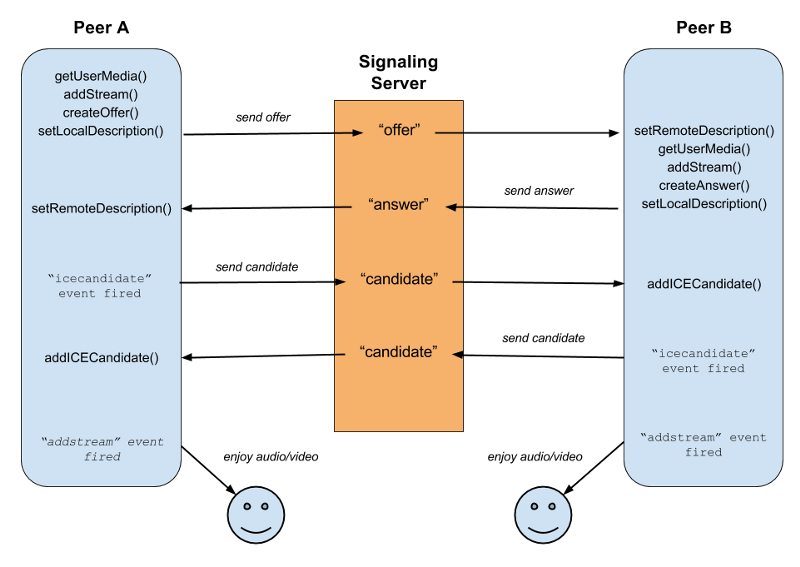
\includegraphics[width=375px]{signaling.png}
	\caption{WebRTC signaling flow}
\end{figure}

\subsection{STUN server}

A Session Traversal Utilities for NAT (STUN\footnote{\url{https://tools.ietf.org/html/rfc5389}}) server is a service that provides a tool for hosts to discover the presence of a NAT, and to discover the mapped, usually public, IP address and port number that the NAT has allocated for the application's flows to remote hosts. This service basically checks the \verb|IP:port| of an incoming request and responds that combination back.

On the gathering candidates process of ICE, STUN servers will be used to gather the public IP and port of the device, so it can be accessed from outside the local network (otherwise ICE would only provide local directions).

\begin{figure}[ht!]
	\centering
	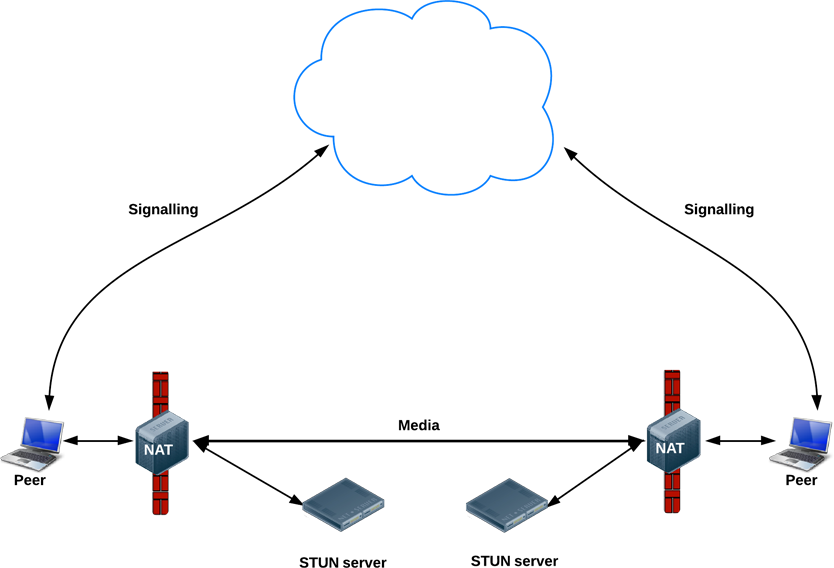
\includegraphics[width=375px]{stun.png}
	\caption{STUN server operation, courtesy of html5rocks.com}
\end{figure}

\subsection{TURN server} 

There are some cases in which media cannot be directly transmitted between peers (typically, on complex networks with NATs and firewalls). In that case, WebRTC uses what's called a Traversal Using Relays around NAT (TURN\footnote{\url{https://tools.ietf.org/html/rfc5766}}) server, which basically acts as a relay which forwards data (audio/video, not signaling data) between peers. 

It's worth noting that every TURN server supports STUN as well.

\begin{figure}[ht!]
	\centering
	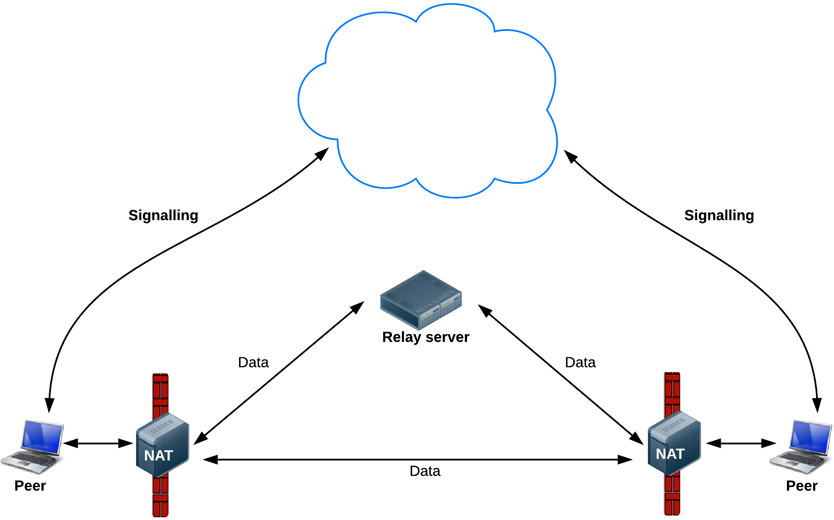
\includegraphics[width=375px]{dataPathways.png}
	\caption{TURN data paths, courtesy of html5rocks.com}
\end{figure}

\section{Related work}

For WebRTC, it's quite unusual to operate completely serverless (mainly because of the lack of complexity and cost of running a pre-build Signaling/STUN/TURN server). There are a few examples, though: 

\begin{itemize}
	\item A trivial example, where two clients live inside the same browser window\footnote{\url{https://webrtc.github.io/samples/src/content/peerconnection/pc1/}}. They communicate from inside the browser and therefore they don't need any external server.
	\item Completelly serverless example\footnote{\url{https://github.com/cjb/serverless-webrtc}}, where users are in different computers but they are responsible for WebRTC offer/answer exchange. 
\end{itemize}

For the implementation of this project, the following solutions have been used as a basis:

\begin{itemize}
	\item Coturn\footnote{\url{https://github.com/coturn/coturn}}. Packaged STUN and TURN server ready to deploy in a computer, based on rfc5766-turn-server by Google.
	\item Stund\footnote{\url{https://github.com/gortc/stund}}. STUN server completely implemented in Go.
\end{itemize}

\section{Background}

This whole project is built in top of WebRTC. WebRTC does not implement (nor includes in the standard) signaling, STUN and TURN, and the available APIs simply expect a certain way to interact with with those components. 

WebRTC provides relatively easy to use APIs that enable media capture and streaming from the web browser, and all the necessary machinery for establishing the peer connection. The only caveat is that the API is not especially flexible when it comes to specifying something different than a standard STUN and TURN servers. In the signaling part, it only requires that it's able to send and receive messages.

Signaling is based in Peerster, a gossip network implemented in class.

\section{Design and architecture}

Users make calls and interact with other users through a web-based UI using a modern browser. At the same time, the user is a node in the gossip network. Both tasks (serving the static content of the web page and interacting with other gossip nodes) are accomplished by a single program running locally on the computer.

Therefore, two different parts arise: front-end (user interface) and back-end (signaling, STUN and TURN).

\subsection{Front-end client (browser)}

The WebRTC client is built entirely in HTML5, CSS3 and JS. Unlike other similar messaging services, it does not require the installation of any browser plugin and it's multiplatform. The UI consists of a single web page that has two states:

\begin{itemize}
	\item \textbf{In active call}. The user is in a call with another user, so it can see the other's audio/video feed as the main object in the window and its own in a smaller box. Users can switch the webcam video feed for the video of the computer screen. They can send files and text messages using the chat as well. Finally, they can terminate the call.
	\item \textbf{Not in active call}. In that case, the user sees a list of known users (real user names, not necessarily directly connected with the peer), which can be clicked to initiate a new call. At the same time, the user can receive a call from another user, which then can be accepted or rejected. Then, the user can open an advanced options dialog which shows the known peers (\verb|IP:port| combinations of nodes directly connected) and the possibility to add a new one. Finally, the user can enable or disable the usage of a TURN server.
\end{itemize}

If for some reason communication is interrupted (one peer is down, network connection is not reliable, there's a hardware failure with the webcam...) the call will be ended and both users will be returned to the \textit{not in active call} state, in which they can redo the call.

All four major communication functionalities (audio/video, text chat, file transfer and screen sharing) rely only on WebRTC technologies and not in the previous implementation of Gossiper, because they are more reliable, fast and secure (communication is peer to peer and encrypted). 

The communication between the browser and the server (running process) is done first by standard HTTP requests and responses (for serving the static files) and then, by WebSockets (for updating the page information dynamically in a more efficient way than polling).

\subsection{Back-end server (Gossiper)}

The back-end consists of three parts: the gossip client, the STUN server and the TURN server. 

The idea is propagate signaling data between nodes in the form of private messages between gossip peers. 

For the STUN and TURN parts, instead of modifying the internals of WebRTC\footnote{The fact that the WebRTC API is quite simple and abstracted means that modifying the internal behavior is painful, therefore, using the proposed implementation achieves the same result without dark modifications on the client code.}, a list of servers is given to the ICE engine on each client, and the protocol is already able to establish a connection using various servers. Therefore, each node has a completely standard STUN and TURN instance running in parallel with the gossiper.

Here is a detailed explanation of the design of each component:

\subsubsection{Gossiper (signaling)}

With signaling, there are two steps: first is peer discovery, which is already implemented in Gossiper (nodes know each other and know a direct path between them). Second, is the exchange of metadata for the call, which is sending and receiving offers and answers in SDP format. Since that can be easily modeled and encoded in Protobuf, the exchange is just a matter of sending Gossiper private messages between peers.


\subsubsection{STUN}

The STUN server is integrated in the binary as well. In a separate process, it listens to the default STUN port (\verb|3478|) for queries and behaves in the standard way.

\subsubsection{TURN}

Due to lack of proper Go implementations (the ones tested did not work properly), TURN server must be launched as a separate process using a packaged TURN server (Coturn has been used for this implementation). TURN server must listen in the default TURN port (\verb|3478|) as well.

\section{Implementation}

\subsection{Launching the program}

The main program that contains the web server, the gossiper node and the STUN server is implemented in Go and can be compiled into a single binary. Therefore, executing \verb|go build| on the project's root folder and then \verb|./decWebRTC -name=nodename| is enough for having it running.

The full command line options of the program are the following:

\begin{verbatim}
-disableGui
    	Disable GUI
  -gossipPort int
    	Port in which gossips are listened (default 5000)
  -guiPort int
    	Port in which the GUI is offered (default 8080)
  -name string
    	Name of the node
  -peers string
    	List of peers
  -rtimer int
    	How many seconds the peer waits between two route rumor messages 
    	(default 10)
\end{verbatim}

To execute the optional TURN server, it suffices with a default installation of Coturn, please refer to the instructions of its website to do so\footnote{\url{https://github.com/coturn/coturn/wiki}}.

\subsection{Access to the GUI}

Once the main program is running, users can access to the GUI (unless the \verb|-disableGui| option has been specified, in which case the node will simply act as a intermediate node for allowing communication of others). To do so, they have to open a browser and navigate to \verb|https://127.0.0.1:8080|.

Notice that the page is served in the \verb|localhost| but using \verb|HTTPS|. That is because most of WebRTC implementations impose restrictions on which kind of data (especially webcam and microphone) and which permissions can be granted over non-secure webpages. To implement so, a self-signed certificate is generated (and included with the source code), so an exception to the browser must be added as well.

The system is designed to accept only one GUI instance (a browser tab) per node, so messages can be easily forwarded. In case that a new tab is opened when there's already one, a message will be shown and no functionality will work. In case of receiving an incoming call and having none opened GUI tabs, the call will be rejected and the originating user will get a message informing of it.

The GUI has been implemented using Bootstrap\footnote{\url{https://getbootstrap.com/docs/3.3/}} as a front-end CSS framework and jQuery\footnote{\url{http://jquery.com}} for prebuilt javascript utilities.

\begin{figure}[ht!]
	\centering
	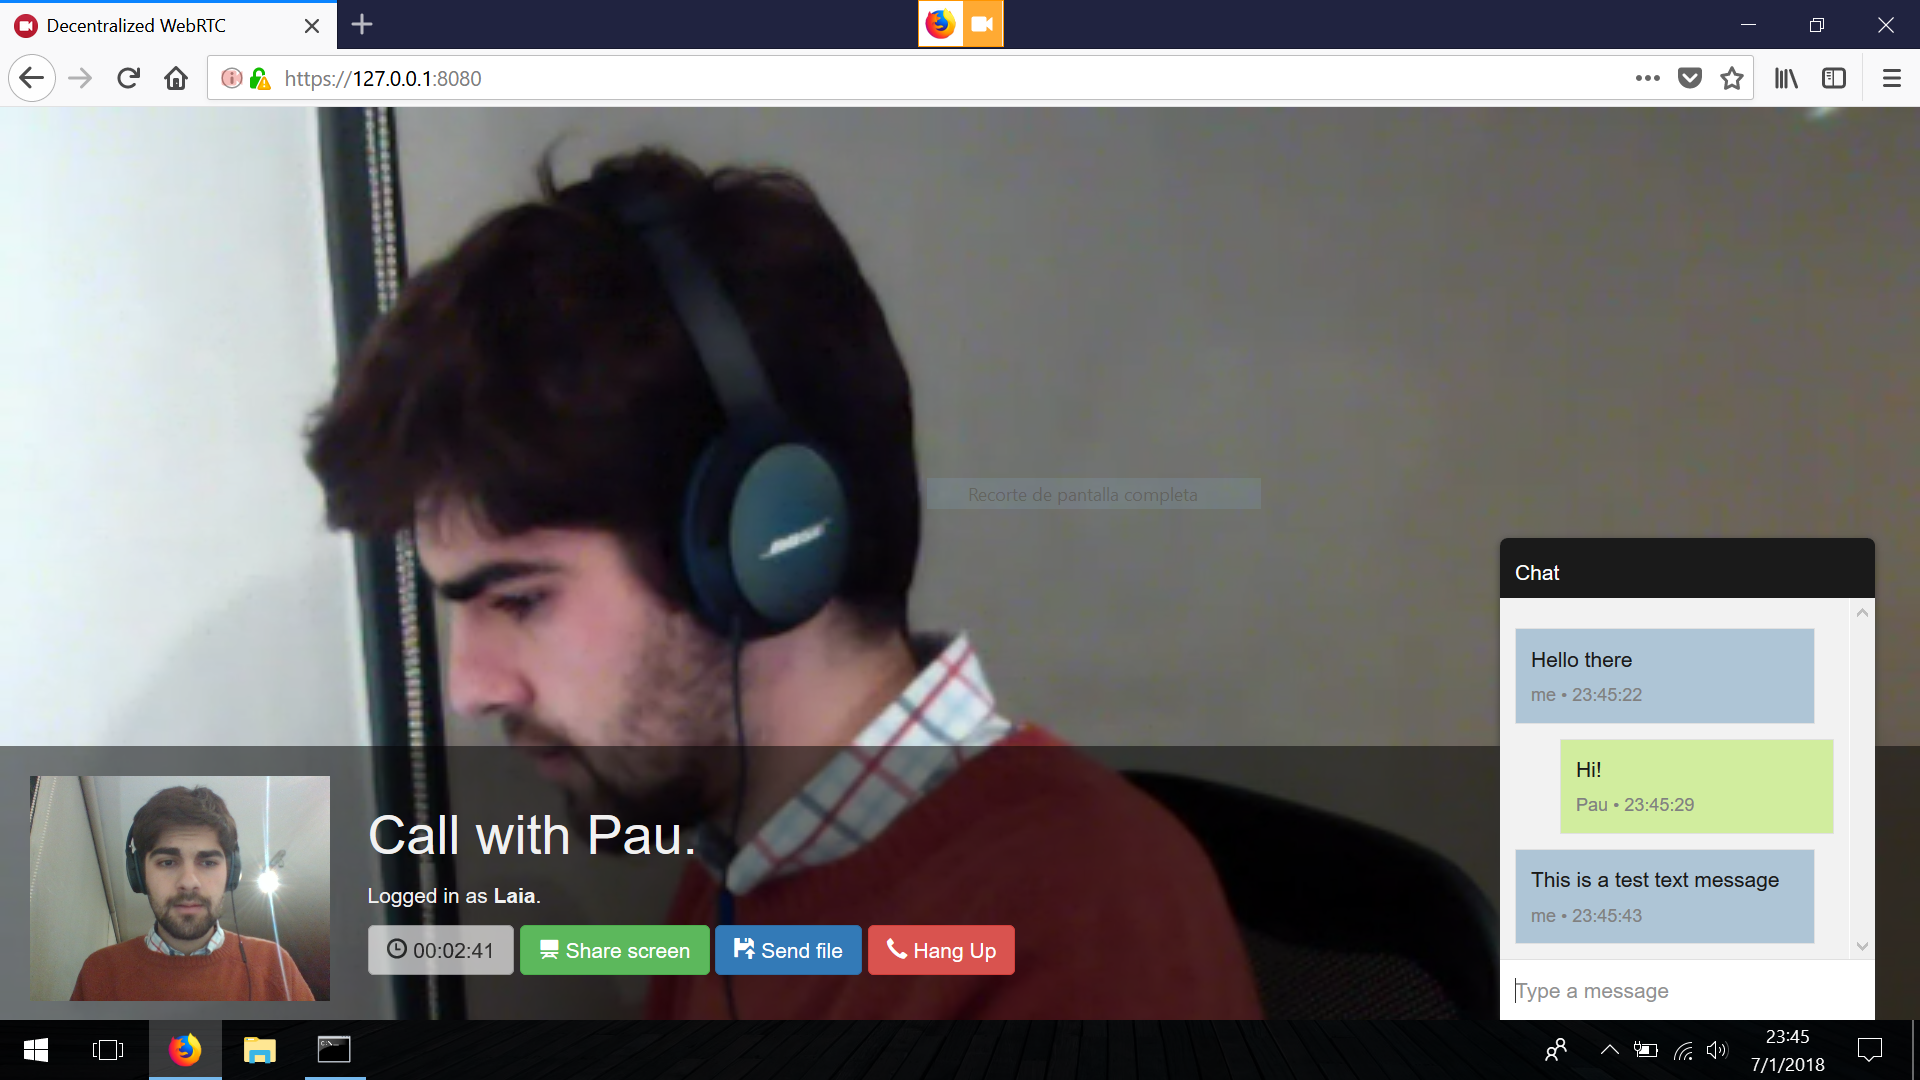
\includegraphics[width=420px]{full-screen.png}
	\caption{Screenshot of the main UI while in a call}
\end{figure}

\begin{figure}[ht!]
	\centering
	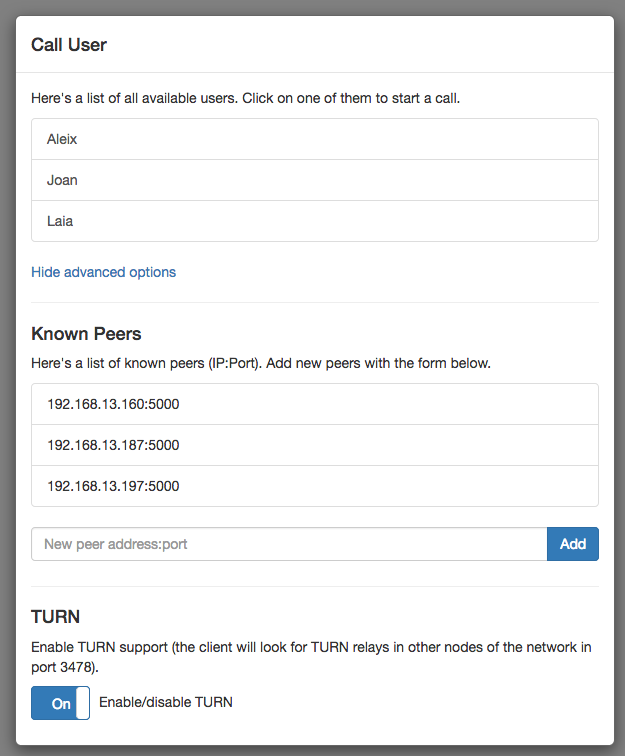
\includegraphics[width=250px]{user-selection.png}
	\caption{User selection and advanced options when not in active call}
\end{figure}

\subsection{Call procedure}

\begin{figure}[ht!]
	\centering
	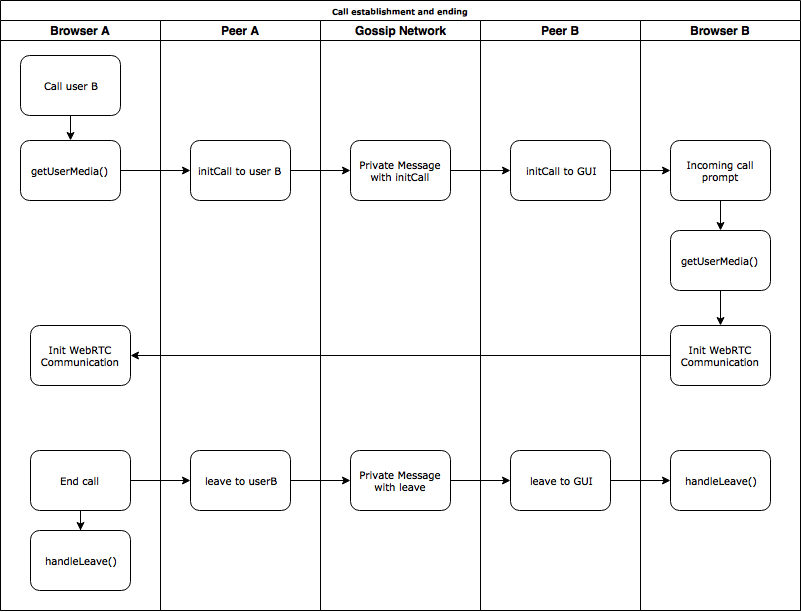
\includegraphics[width=420px]{call-establishment-ending.png}
	\caption{Call establishment and ending procedures}
\end{figure}

When the page is opened, no media permission is requested to the user (this can be noted by the fact that for instance, the webcam LED is turned off). Media can be requested (via \verb|getUserMedia| browser routine) in two different scenarios:

\begin{itemize}
	\item \textbf{User sends a call request to another user}. The browser media prompt is shown and if all permissions are given and there is no error while accessing the hardware, the communication is started.
	\item \textbf{User receives a call request from another user}.When an init call request is received from another user, a prompt is shown for accepting or ignoring the call. If the call is accepted, then the media prompt is shown.
\end{itemize}

Once both users have granted media permissions, the WebRTC communication is started. It is actually the peer that receives the call who starts the communication. Figure 7.3 contains a diagram with the whole flow of establishing and ending a call (WebRTC specifics and media transmission have been omitted since they appear in figure 3.1).

If for some reason media permissions are not granted or the call is directly rejected, a \verb|leave| message is sent to the other peer so it stops gathering video and returns to the initial state. This happens as well when some user presses the hang up button.

\begin{figure}[ht!]
	\centering
	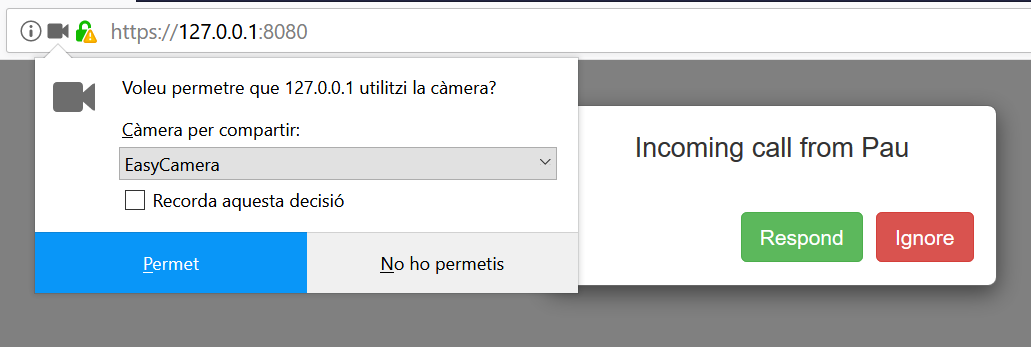
\includegraphics[width=350px]{incoming-call.png}
	\caption{Incoming call with user permission dialog}
\end{figure}

When the call is started, a clock with the elapsed time is displayed and active in the window. When the call ends or resets, the clock does it as well.

Since the WebRTC API is still inestable (especially between browsers, where prefixes such as \verb|webkit-| or \verb|moz-| are quite usual), the adapter.js\footnote{\url{https://github.com/webrtc/adapter}} library has been used.

\subsection{Peer interaction}

During the call, the following are established:

\begin{itemize}
	\item \textbf{RTCPeerConnection}. This is a standard WebRTC peer to peer connection which carries audio and video between the peers as well as metadata about the call.
	\item \textbf{Send Channel (DataChannel)}. Data channel used for sending text messages and files to the other peer.
	\item \textbf{Receive Channel (DataChannel)}. Data channel user for receiving text messages and files to the other peer.
\end{itemize}

\begin{figure}[ht!]
	\centering
	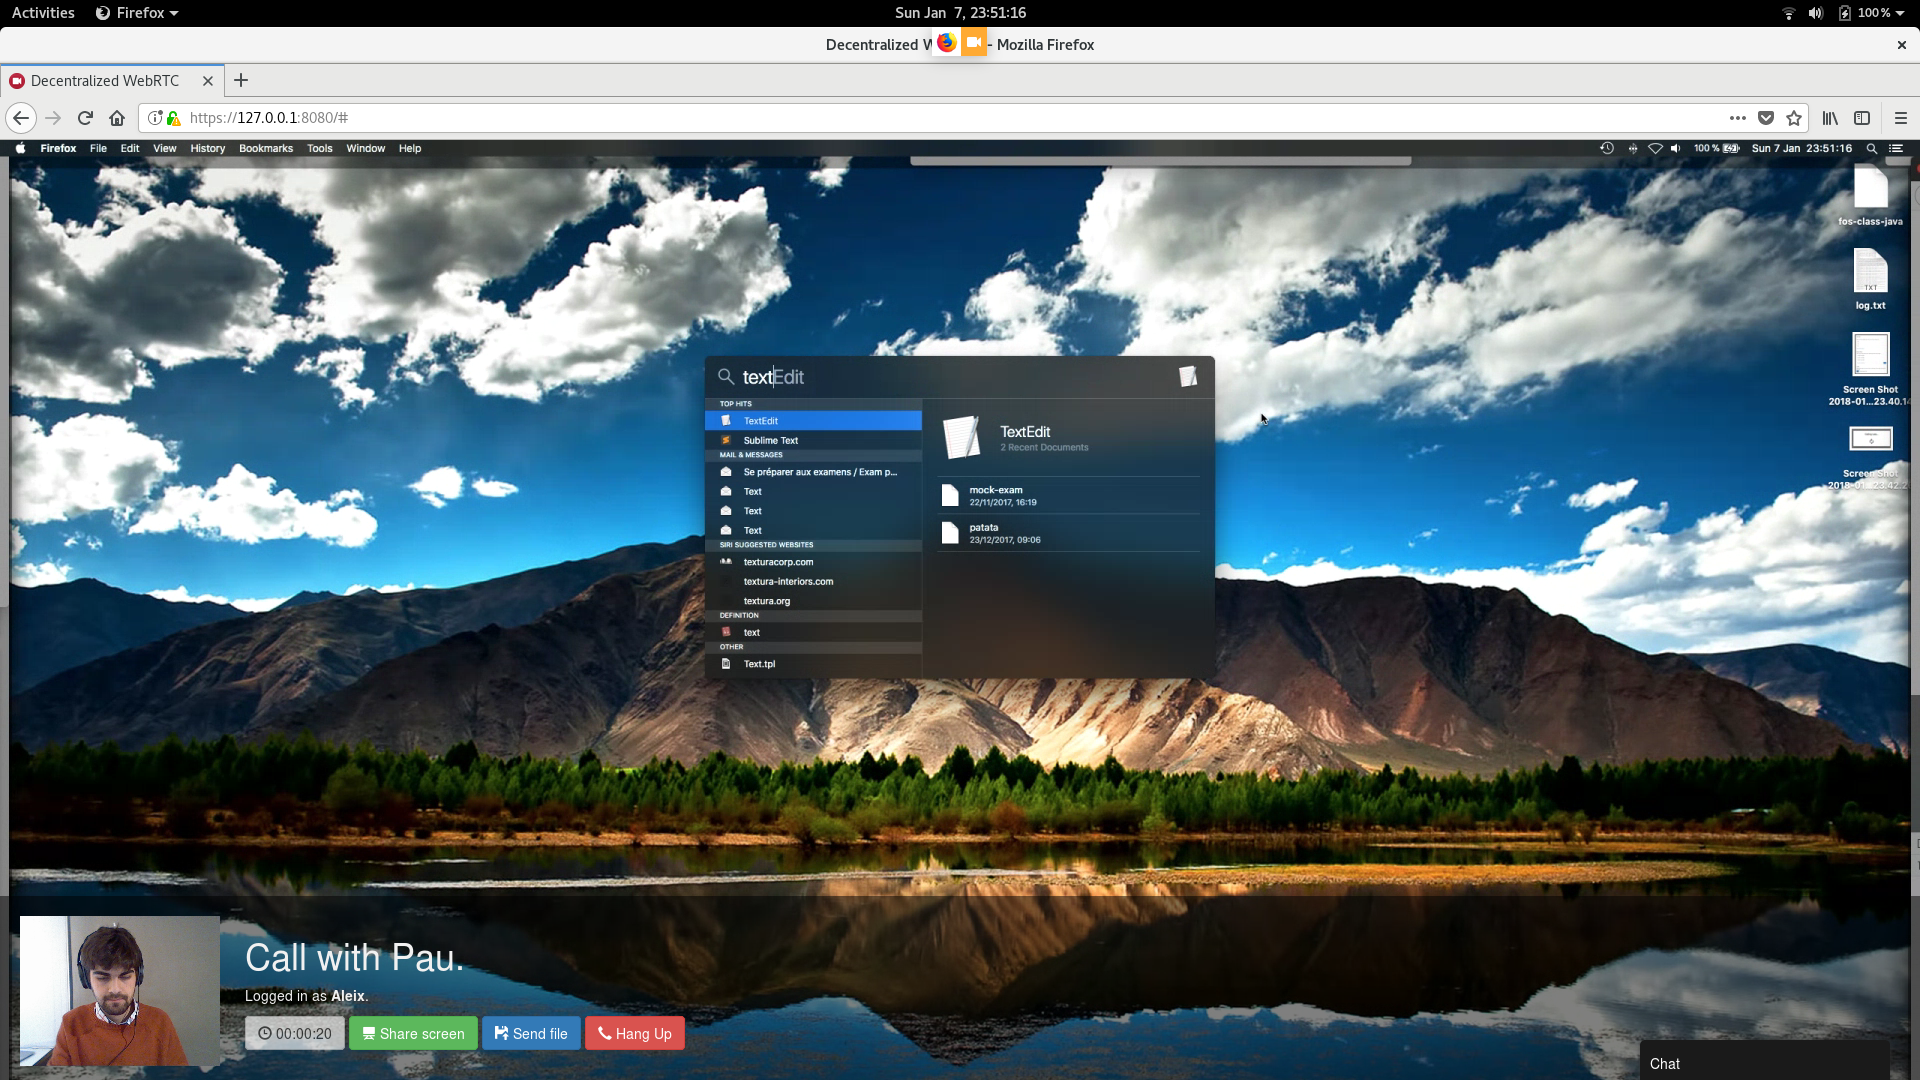
\includegraphics[width=420px]{screen-sharing.png}
	\caption{Call with one user sharing its screen}
\end{figure}

The default view contains the peer's video in full screen and a miniature of user's video. On top of that there are some controls that enable the other kinds of interaction:

\begin{itemize}
	\item By clicking \textit{share screen}, the own user's video feed (miniature) switches to the current view of the screen, and on the other side, the main video input becomes the screen as well. This is done assigning the main video stream to the webcam or the screen (using \verb|replaceTrack| on the browser).
	\item The chat tab on the bottom right of the window opens a traditional text chat, which displays messages in real time in chronological order. It also allows the user to send private messages to the partner by a text form. Those messages are sent through the data channel in \verb|JSON| format.
	\item The file sharing button opens a modal with a standard HTML form for file upload. Once the file is uploaded, it is splitted in chunks of 16k\footnote{The maximum recommended size for WebRTC data channels}. Then, a metadata JSON (containing filename, size, type...) is generated and sent to the peer so it can reconstruct the file. Then, all chunks are sent through the data channel as well.
\end{itemize}

\begin{figure}[ht!]
	\centering
	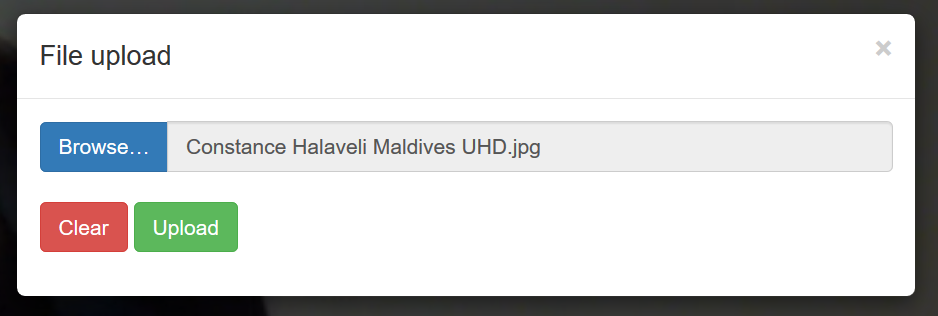
\includegraphics[width=350px]{file-upload.png}
	\caption{File upload dialog}
\end{figure}

\begin{figure}[ht!]
	\centering
	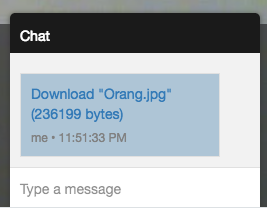
\includegraphics[width=250px]{file-download.png}
	\caption{Downloaded file in the chat}
\end{figure}

\subsection{Communication front-back}

Static files (HTML, CSS, JS and images) are served when the page is requested using a standard Go routing \verb|ListenAndServeTLS|. Then, a Websocket connection is established, using the \verb|WebSocket| object in the front-end and the Gorilla Websocket\footnote{\url{https://github.com/gorilla/websocket}} library on the back-end. 

All messages transmitted through the socket are encoded as JSON messages.

\subsection{Modifications to Peerster}

Although the Gossip network is based in the Peerster implementation done in class (after HW3), some modifications have been introduced to make it fit properly to the presented usecase:

\begin{enumerate}
	\item \textbf{Simplified messages}. Now there are only three kinds of messages: route rumors for discovering routes between nodes, private messages carrying actual data and status messages for keeping vector clocks in sync.
	\item \textbf{Not storing messages}. Since rumors no longer contain information, they are not stored. In case someone requests them, they can be reconstructed (they only contain \verb|LastIP| and \verb|LastPort| which are stored for every peer in an internal data structure).
	\item \textbf{Rumor messages, private messages and file sharing removed}. All these user-faced features are now removed, since they are replaced (except for rumor messages) by better WebRTC-based implementations.
	\item \textbf{CLI removed}. All UX is now focused in the GUI, so the CLI is removed as well. The UDP listener needed for it is removed as well.
	\item \textbf{Peer propagation}. If it is reachable, the direction contained in \verb|LastIP| and \verb|LastPort| will be added to the known peers list.
	\item \textbf{Peer deletion}. When a peer cannot be reached (directly or indirectly), is now deleted from the known peers, with all of its related known data.
	\item \textbf{Listen to all directions}. Instead of binding the UDP listener to an IP and a port, now it's binded to \verb|0.0.0.0:port|.
\end{enumerate}

\subsection{STUN implementation}

A STUN server is wrapped inside the main binary, which is basically a port of stund. It works as a regular STUN server and listens to queries in the default STUN port (this cannot change, otherwise other nodes on the network would not find it).

This kind of solution has been chosen by the simplicity of the implementation and the fact that since it's Go code, can interact with the rest of the application.

\section{Evaluation}

The evaluation plan to test the implementation consists on testing two things: that the communication functionalities during the call work properly (audio, video, file sharing, chat) and that users can establish configurations on different network topologies.

Therefore, the same test will be carried in five different network configurations, and the user experience should be the same (or at least, quite similar) regardless of the case. The steps that will be followed in each case will be:

\begin{enumerate}
	\item Launch all necessary instances and wait a short amount of time (30 secs) for all users to appear as visible to each other.
	\item Start a call from user A to user B, granting all permissions to get media devices.
	\item Accept the call on user B.
	\item Wait for the video to appear on both sides (it should take less than 5 secs).
	\item Check that the video and audio has no noticeable lag and that the quality is the best allowed by each webcam (usually 480-720p).
	\item Send a few text messages using the chat between the two peers and check they arrive well-formatted to the other side.
	\item Send a \verb|.pdf|, a \verb|.png| and a \verb|.txt| file and check it arrives well-formatted to the other side.
	\item Share screen and check that video changes to it, it's stable and the whole screen is displayed.
	\item End call and check it nicely ends (shuts down video and returns to initial state) on both sides.
\end{enumerate}

A stable network connection is assumed for all peers. If that wasn't the case, the system first degrades the audio/video quality (this is done by the ICE framework), and if it's completely lost, it ends the call.

All tests have been conducted using the latest stable version of Mozilla Firefox (57.0.4) in laptops running macOS 10.13, Linux (Fedora Workstation 27) and Windows 10.

The network configurations chosen are represented in the following figures (from 1 to 5). Straight lines represent physical connections between devices. Dotted lines represent connections between gossiper nodes. Users (latptops and desktops) represent nodes with media equipment installed and GUI activated. Servers represent gossip nodes without GUI.

\begin{figure}[ht!]
	\centering
	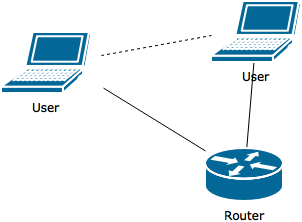
\includegraphics[width=200px]{network-config-1.png}
	\caption{Network configuration 1}
\end{figure}

\begin{figure}[ht!]
	\centering
	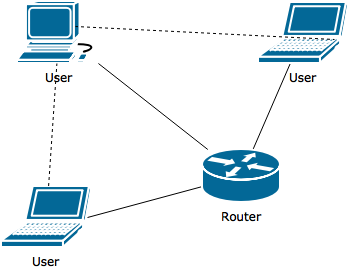
\includegraphics[width=200px]{network-config-2.png}
	\caption{Network configuration 2}
\end{figure}

\begin{figure}[ht!]
	\centering
	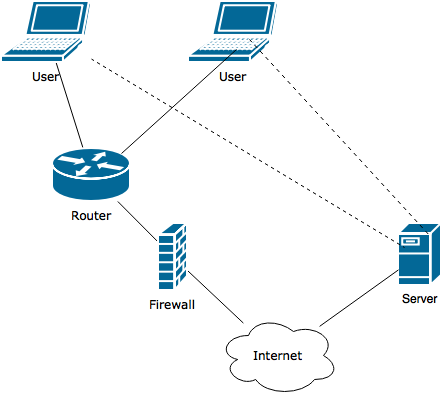
\includegraphics[width=300px]{network-config-3.png}
	\caption{Network configuration 3}
\end{figure}

\begin{figure}[ht!]
	\centering
	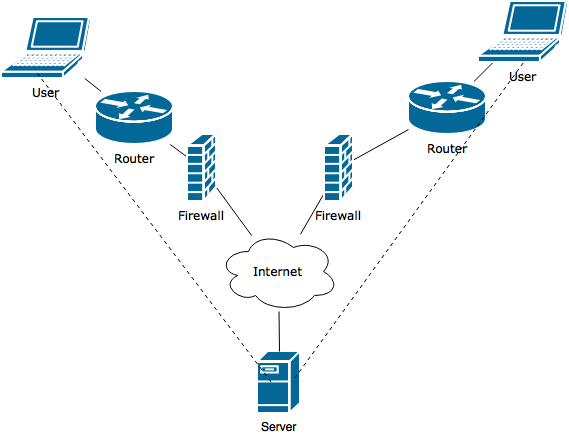
\includegraphics[width=350px]{network-config-4.png}
	\caption{Network configuration 4}
\end{figure}

\begin{figure}[ht!]
	\centering
	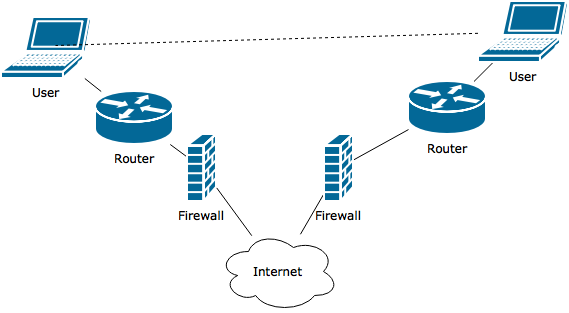
\includegraphics[width=300px]{network-config-5.png}
	\caption{Network configuration 5}
\end{figure}

\end{document}